\documentclass[12pt]{article}
\usepackage[margin=2.5cm]{geometry}
\usepackage{enumerate}
\usepackage{amsfonts}
\usepackage{amsmath}
\usepackage{fancyhdr}
\usepackage{amsmath}
\usepackage{amssymb}
\usepackage{amsthm}
\usepackage{mdframed}
\usepackage{graphicx}
\usepackage{subcaption}
\usepackage{adjustbox}
\usepackage{listings}
\usepackage{xcolor}
\usepackage{booktabs}
\usepackage[utf]{kotex}

\definecolor{codegreen}{rgb}{0,0.6,0}
\definecolor{codegray}{rgb}{0.5,0.5,0.5}
\definecolor{codepurple}{rgb}{0.58,0,0.82}
\definecolor{backcolour}{rgb}{0.95,0.95,0.92}

\lstdefinestyle{mystyle}{
    backgroundcolor=\color{backcolour},
    commentstyle=\color{codegreen},
    keywordstyle=\color{magenta},
    numberstyle=\tiny\color{codegray},
    stringstyle=\color{codepurple},
    basicstyle=\ttfamily\footnotesize,
    breakatwhitespace=false,
    breaklines=true,
    captionpos=b,
    keepspaces=true,
    numbers=left,
    numbersep=5pt,
    showspaces=false,
    showstringspaces=false,
    showtabs=false,
    tabsize=1
}

\lstset{style=mystyle}

\begin{document}
\title{CSC148 Assigment 1}
\author{Hyungmo Gu}
\maketitle

\section*{1) Get the starter code and read the documentation}
\begin{enumerate}[1.]
    \item Download the zip file that contains the starter code here a1.zip
    \item Unzip the file and place the contents in pycharm in your a1 folder (remember to set your a1 folder as a sources root)
    \item You should see the following files:
    \begin{itemize}
        \item \textit{course.py}
        \item \textit{criterion.py}
        \item \textit{grouper.py}
        \item \textit{survey.py}
        \item \textit{tests.py}
        \item \textit{example\_tests.py}
        \item \textit{example\_usage.py}
        \item \textit{example\_course.json}
        \item \textit{example\_survey.json}
    \end{itemize}

\end{enumerate}

\bigskip

\noindent For this assignment, you will be required to edit and submit the following files only:

\begin{itemize}
    \item course.py
    \item criterion.py
    \item grouper.py
    \item survey.py
    \item tests.py
\end{itemize}

\bigskip

\noindent If you look at these files you will notice that you have been given the signature
and docstrings for all classes and methods. Read through these docstrings carefully;
they describe how you are expected to implement these classes and methods.

\bigskip

\subsection*{A picture!}

\noindent It might be difficult to imagine how all the classes defined in these files will
interact before you start writing the code itself. To help you out, here is a
diagram of all the classes you will be asked to contribute to for this assignment:

\begin{center}
    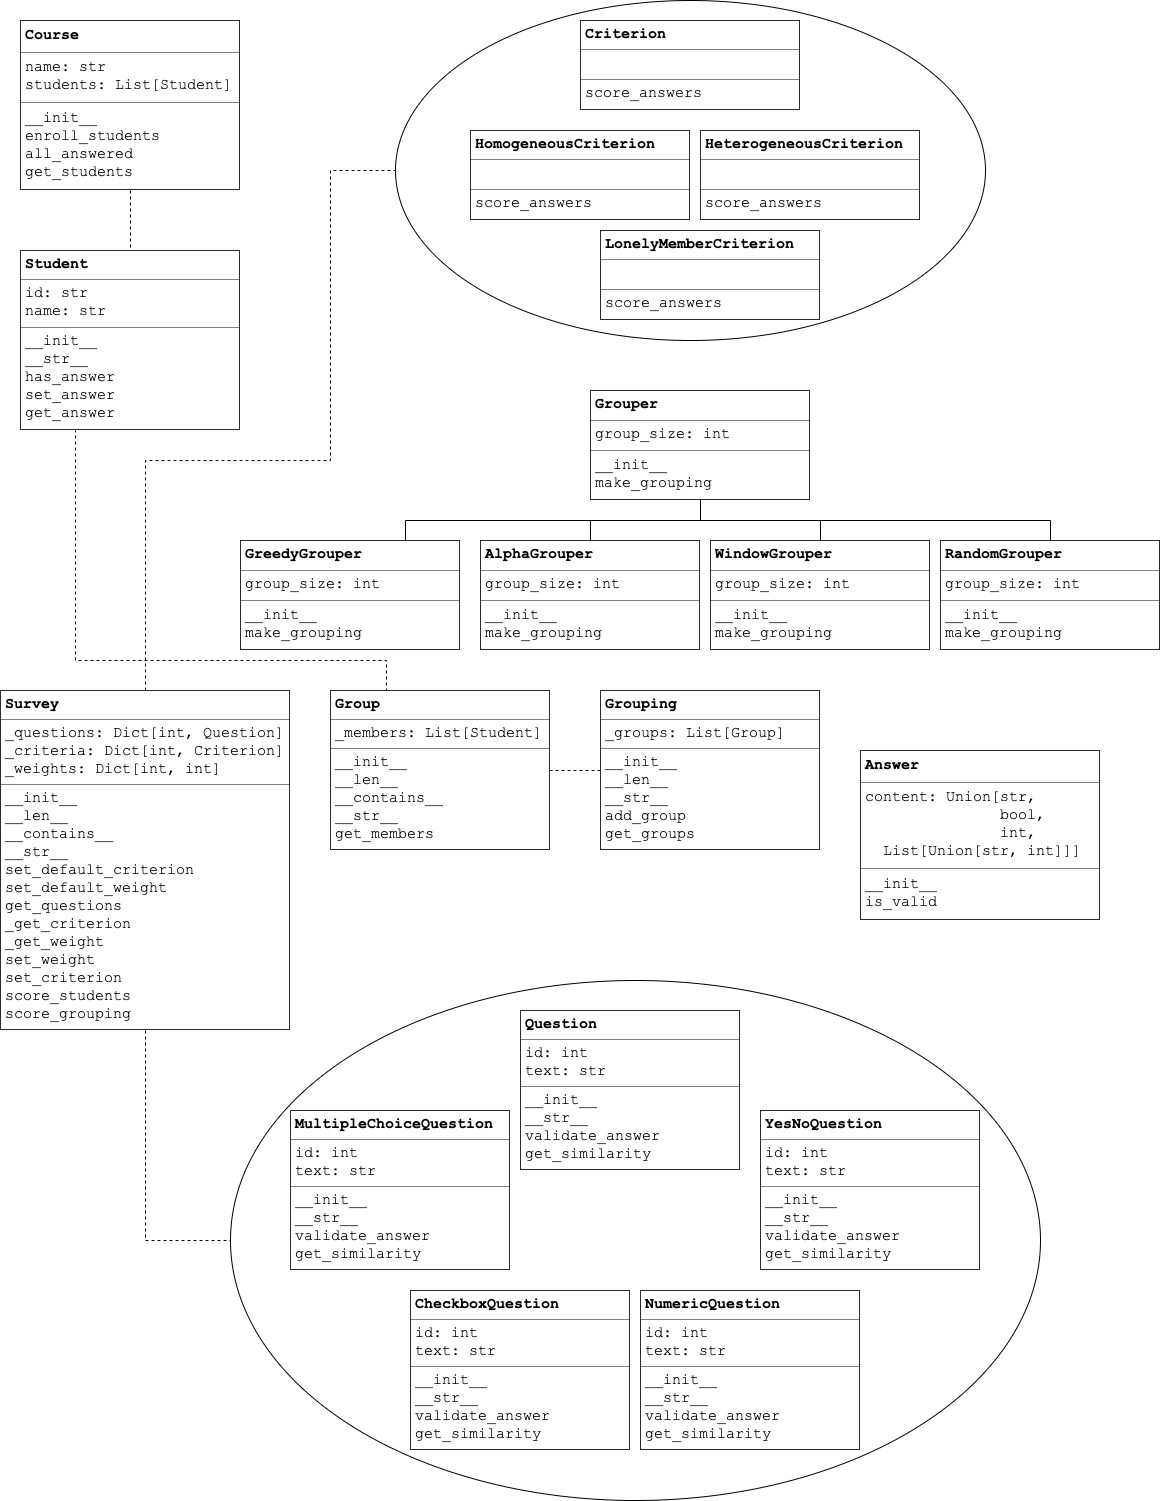
\includegraphics[width=0.8 \linewidth]{images/assignment_1/image_1.png}
\end{center}

\noindent Note that the attributes and methods shown in this diagram are only the ones
that we have given you in the starter code. You may need to define additional
private attributes or private helper methods.

\subsection*{Legend:}

\begin{itemize}
    \item dashed lines indicate a composition relationship between classes
    \item solid lines indicate an inheritance relationship between classes
    \item a solid circle around a group of classes indicates that there exists an inheritance relationship between these classes but it is not defined (you get to decide!)
\end{itemize}

\bigskip

\subsection*{Test your code!}

\begin{itemize}
    \item Try running the example\_tests.py file: all of the tests should fail because you haven’t written any code yet!
    \item Try running example\_usage.py file: you should get an error since you haven’t written any code yet!
    \item Open up the tests.py file: it is empty! This is where you will be writing all of your tests for this assignment
\end{itemize}

\subsection*{Something to think about!}
Unlike A0, you will be submitting code split across multiple files. Open up each
of the files and look at which functions and classes are defined in each file. Why do you think the files were organized
in this way? Is there a different way we could have organized these files?

\section*{2) Complete the Student Class}
The Student class represents a student who can be enrolled in a university
course.

\bigskip

\noindent The starter code for the \textit{Student} class can be found in \textit{course.py}. Open up this
file and read through the docstrings for each of the the \textit{Student} class’s methods.
Then, implement each of the methods in the \textit{Student} class.

\bigskip

\noindent Remember: you may need to define additional private attributes or
private helper methods!

\bigskip

\subsection*{Test your code!}
\begin{itemize}
    \item Write at least one unit test for each method in \textit{Student}. You are not
    required to write tests for initializers.
    \item You should write these tests in the \textit{tests.py} file.
    \item Once you have finished writing these tests, run all the tests in \textit{test.py}.
    Make sure your code passes all your tests before moving on.
    \item Run the tests in \textit{example\_tests.py}, the tests in the \textit{TestStudent} class should now pass.
\end{itemize}

\bigskip

\subsection*{Something to think about!}
The \textit{Student.has\_answer} method asks you to check if a student has a
valid answer to a given question. Do we have a way to determine if an answer is
valid or not yet? Answer: no and we won’t until we complete step 4. You may need
to come back and finish this method after completing step 5.

\section*{3) Complete the Course Class}
The \textit{Course} class represents a university course.

\bigskip

\noindent The starter code for the \textit{Course} class can be found in \textit{course.py}. Open up this
file and read through the docstrings for each of the the \textit{Course} class’s methods.
Then, implement each of the methods in the \textit{Course} class. You may find the
function \textit{sort\_students} helpful.

\bigskip

\noindent Remember: you may need to define additional private attributes or
private helper methods!

\subsection*{Test your code!}
\begin{itemize}
    \item Write at least one unit test for each method in \textit{Course}. You are not
    required to write tests for initializers.
    \item You should write these tests in the \textit{tests.py} file.
    \item Once you have finished writing these tests, run all the tests in
    \textit{test.py}. Make sure your code passes all your tests before moving on.
    \item Run the tests in \textit{example\_tests.py}, the tests in the \textit{TestCourse} class
    should now pass.
    \item Something to think about!
    \item The \textit{Course.all\_answered} method asks you to check if all students have
    a valid answer for every question in a \textit{Survey}. Which steps do you need to
    complete before you can finish this method? You may have to come back later to
    finish the \textit{Course.all\_answered} method.
\end{itemize}

\section*{4) Complete the Question Classes}

\section*{5) Complete the Answer Class}

\section*{6) Complete the Criterion Class}

\section*{7) Complete the Group Class}

\section*{8) Complete the Grouping Class}

\section*{9) Complete the Survey Class}

\section*{10) Complete the helper functions in \textit{grouper.py}}

\section*{11) Complete the Grouper Classes}

\section*{12) Test the Code Again}

\section*{13) Submit your work}

\end{document}